\documentclass[brazil]{abnt}
\usepackage[utf8]{inputenc}
\usepackage[brazil]{babel}
\usepackage{listings}

\usepackage{courier}
 \lstset{
         basicstyle=\footnotesize\ttfamily, 
         numberstyle=\tiny,          
         numbersep=5pt,              
         tabsize=2,                  
         extendedchars=true,         
         breaklines=true,            
         keywordstyle=\color{red},
                frame=b,         
         stringstyle=\color{white}\ttfamily, 
         showspaces=false,           
         showtabs=false,             
         %xleftmargin=17pt,
         %framexleftmargin=17pt,
         %framexrightmargin=5pt,
         %framexbottommargin=4pt,
         %backgroundcolor=\color{lightgray},
         showstringspaces=false      
 }
 \lstloadlanguages{
         %[Visual]Basic
         %Pascal
         %C
         C++
         %XML
         %HTML
         %Java
 }

\usepackage{color}
\usepackage{xcolor}
\usepackage{graphicx}
\usepackage{wrapfig}
\usepackage{xunxos-utp}
\usepackage{caption}
\DeclareCaptionFont{white}{\color{white}}
\DeclareCaptionFormat{listing}{\colorbox{gray}{\parbox{0.98\textwidth}{#1#2#3}}}
\captionsetup[lstlisting]{format=listing,labelfont=white,textfont=white}


\makeatletter
\usepackage{babel}
\makeatother
\begin{document}

\autor{Renato dos Santos Cerqueira}
\coautor{Felipe Pedrosa Martinez}
\titulo{Title Placeholder}
\orientador{Adriano Joaquim de Oliveira Cruz}
\comentario{Monografia apresentada para obtenção do Grau de Bacharel em Ciência da Computação pela Universidade 
Federal do Rio de Janeiro.}
\instituicao{Departamento de Ciência da Computação \par Instituto de Matemática \par Universidade Federal do Rio de Janeiro}
\local{Rio de Janeiro - RJ, Brasil}
\data{21/12/2012}

\Ncapa
\NFolhaDeRosto

\begin{folhadeaprovacao}
Monografia de Projeto Final de Graduação sob o título \textit{``\ABNTtitulodata''},
defendida por \ABNTautordata~e \ABNTcoautordata~e aprovada em \ABNTdatadata, no Rio de Janeiro,
Estado do Rio de Janeiro, pela banca examinadora constituída pelos
professores: \setlength{\ABNTsignthickness}{0.4pt}

\assinatura{Prof. Ph.D. Adriano Joaquim de Oliveira Cruz\\ Orientador} \assinatura{???\\ Universidade ???} \assinatura{???\\ Universidade ???}
\end{folhadeaprovacao}

\begin{resumo}
O objetivo deste trabalho é fazer um \textit{engine} de jogo para o \textit{videogame Nintendo DS\texttrademark} e também um editor de fases 
e configurações, como seria feito numa equipe de desenvolvimento de um jogo comercial, dando a possibilidade aos \textit{designers} 
de fazerem seus \textit{sprites} e criarem as fases com eles, sem que fosse necessário mexer com códigos.
\end{resumo}

\begin{abstract}
The objective of this paper is to make a game engine to the Nintendo DS\texttrademark system and a level and configurations editor, as it
would be done in a development team in a comercial game, giving designers the possibility to make their sprites and create their levels 
without touching actual source code.
\end{abstract}

\chapter*{Dedicatória}

\chapter*{Agradecimentos}

\tableofcontents{}
\listoffigures
\listoftables

\chapter{Introdução\label{cap:introducao}}

\vfill{}
\begin{flushright}{}``\emph{Quote 1}''\\
{\small Author1}\end{flushright}{\small \par}
\vfill{}

Neste capítulo são apresentados o objetivo desta monografia e a estrutura
da mesma.
\newpage


\section{Objetivo deste trabalho}

A área de jogos eletrônicos é uma área relativamente nova, se comparada a outros ramos da ciência da computação. No entanto, por mais que compreenda conceitos importantes de computação, engloba outros que fogem ao seu escopo. Para o desenvolvimento de um jogo eletrônico, além de conhecimentos de linguagens de programação, algoritmos e estruturas de dados, interface humano-computador, inteligência artifical, etc; é preciso considerar aspectos mais subjetivos que dizem respeito a um jogo de forma geral, seja ele eletrônico ou não. O gameplay, ou a mecânica do jogo, ou seja, a forma com que o jogo vai se desenrolar e o seu funcionamento, é um exemplo claro de que o seu desenvolvimento e sua concepção vão muito além do que pode ser programado, compilado e executado em um computador.

É possível observar o crescimento da área se notarmos que o primeiro exemplo conhecido de jogo eletrônico aparece em 1947, quando Thomas T. Goldsmith Jr. e Estle Ray Mann introduziram sua patente para um Dispositivo de Entretenimento usando Tubo de Raios Catódicos em \\\cite{2455992}. Quando vemos jogos produzidos na época do Atari 2600 e Magnavox Odyssey, estes eram criações de um único desenvolvedor, muitas vezes em períodos curtos de tempo, sem nem ao menos identificar o time de desenvolvimento. Era comum a aparição de \textit{Easter Eggs} que os desenvolvedores usavam para tentar identificar a sua criação \cite{PrimeiroDevName}.

Mas observamos que com a tecnologia cada vez mais aprimorada, é possível vermos conceitos básicos que definiam os jogos daquela época serem trocados por formas cada vez mais rebuscadas. Podemos observar o desenvolvimento de novas áreas de jogos, onde antes haviam poucos estilos bem definidos, como corrida, luta e aventura, hoje há muitos mais, há jogos casuais, sociais e de multiplay massivo.

Hoje em dia, a indústria de jogos conta com super~produções com uma quantidade quase infindável de desenvolvedores, designers, criadores de fases, dentre outros tantos profissionais trabalhando cada um com sua especialidade.

Neste trabalho, o que nos propomos a fazer é nos inserir no contexto desses times de criação modernos, vendo apenas uma pequena parte dessa grande cadeia de desenvolvimento: a criação de ferramentas para facilitar a interação entre equipes de ramos diferentes. Mais especificamente, criando um jogo em duas dimensões, do tipo plataforma para o videogame portátil Nintendo DS. Para isso, desenvolvemos uma engine, responsável por controlar todas as partes envolvidas no funcionamento do jogo como áudio, vídeo, estruturas de dados, controle de personagens, fases, itens etc. Parte do nosso objetivo é tornar esta engine  simples e de fácil reutilização. Isto foi feito através de ferramentas de criação e configuração dos componentes pertinentes ao mundo do jogo.

Nos propomos a fazer o papel do desenvolvedor: Criar as ferramentas, imaginando como os outros times as usariam e aprimorando ao máximo para esse fim.

\section{Contexto}

Nos propomos a criar ferramentas para desenvolver jogos em duas dimensões do tipo de plataforma. Mas, o que é exatamente um jogo de plataforma em duas dimensões? Podemos pensar em exemplos clássicos, como Super Mario World para o Super Nintendo, ou Sonic The Hedgehog para o Sega Mega Drive.

Nem todos os jogos plataforma são em duas dimensões. Mas vamos aqui nos focar neles para facilitar o entendimento e o desenvolvimento de soluções. Nessa modalidade, uma característica comum presente em muitos jogos é o uso de \textit{tiles}, figuras de tamanho pré-definido, que compõem todo o mundo. \textit{Tile}, em inglês, significa ladrilho. Além disso, nesse tipo de jogo, todos os objetos costumam ser feitos da combinações de \textit{sprites} e muitas vezes um \textit{sprite} é usado mais de uma vez em diferentes posições, para vários inimigos, por exemplo. Ou seja, os tiles compõem o mundo, como ladrilhos, e os \textit{sprites} o habitam.

Podemos definir um jogo de plataforma 2D por suas características comuns: o jogador controla um personagem que se movimenta para os lados, pode ou não saltar, ter ou não algum tipo de arma e tem como objetivo percorrer uma série de fases derrotando pequenos inimigos, para ao final derrotar algum grande inimigo e recuperar alguma coisa. Claro que essa é uma definição bem aberta, e é nela que vamos tentar nos inspirar ao escrever o motor que será executado no Nintendo DS.

Nosso objetivo é criar uma engine que leia algum tipo de arquivo de configuração, onde estarão detalhadas informações sobre quais são as imagens que compõem o personagem principal (ou personagens, no caso de haver uma escolha); informações sobre os inimigos como por exemplo a qual tipo de movimento ele obedece; descrição dos itens, como por exemplo qual efeito ele causa no personagem principal ou nos inimigos e informações sobre as fases, posicionamento de itens, inimigos e as imagens que as compõem.

\section{Estrutura da monografia}

Escrever aqui a estrutura da monografia.

\chapter{Desenvolvendo para o Nintendo DS\label{cap:hardds}}

\vfill{}
\begin{flushright}{}``\emph{Quote 2}''\\
{\small Author 2}\end{flushright}{\small \par}
\vfill{}

Neste capítulo são apresentados a motivação para desenvolver para a plataforma, as suas especificações e como desenvolver.
\newpage

\section{Motivação}

Há poucos trabalhos desenvolvidos para plataformas diferentes do PC, seja pelo mais restrito número de usuários, menor versatilidade de ferramentas e recursos associados ou mesmo pela maior dificuldade de encontrar documentação relativa ao desenvolvimento. A motivação para este trabalho é, dada essas circunstâncias, criar um facilitador para o desenvolvimento de jogos para um console real, desenvolvendo ferramentas para fomentar uma maior quantidade de trabalhos para a plataforma, apesar das dificuldades.

\section{Especificações}

Nesse trabalho, nos focamos nas duas primeiras iterações do Nintendo DS: o Nintendo DS original, lançado no final de 2004, que normalmente é chamado de ``DS Phat''; e a segunda iteração, o Nintendo DS Lite, lançado no meio de 2006.

Ambos possuem hardware muito parecido, e as maiores diferenças são a estética e o contraste e iluminação da tela. Vamos às especificações:

\noindent{\bf Nintendo DS:}\\
{\bf Peso:} 275 gramas\\
{\bf Dimensões:} 148.7mm x 84.7mm x 28.9mm\\
{\bf Telas:} Duas telas, ambas com 3 polegadas, de LCD TFT (Thin-Film Transistor) com 18-bit de cor, resolução de 256x192. As duas telas tem um espaço entre elas de aproximadamente 21mm, e a tela de baixo possui touchscreen resistivo, que responde a um ponto de pressão por vez, fazendo a média no caso de vários pontos serem pressionados de uma vez.\\
Possui iluminação traseira, que pode ser desligada por software.\\
{\bf Entradas:} Possui duas entradas de cartucho, uma para o formato de cartucho do seu antecessor, o Gameboy Advance(GBA), na parte inferior,e uma para seu próprio formato de cartucho na parte superior.\\
{\bf Processadores:} Possui dois processadores ARM, um ARM946E-S a 67MHz, que é o processador principal, responsável pelo loop de jogo e renderização de vídeo e um coprocessador ARM7TDMI a 33MHz, responsável pelo som, wi-fi, e, quando em modo GBA, diminui seu clock para 16MHz, e passa a ser responsável pelo processamento principal.\\
{\bf Memória:} Possui 4MiB de RAM principal, expansíveis através da entrada de Gameboy Advance, no entanto, essa expansão só foi usada em jogos oficiais pelo Opera Browser.\\
{\bf Wireless:} Possui uma conexão IEEE802.11b, compatível com encriptação por WEP. WPA e WPA2 não são suportadas. Essa conexão também pode ser usada para comunicação entre consoles.\\

\noindent{\bf Nintendo DS Lite:}\\
{\bf Peso:} 218 gramas\\
{\bf Dimensões:} 133mm x 73.9mm x 21.87mm\\
{\bf Telas:} Mesma especificação que o original, no entanto, possui quatro níveis de iluminação que podem ser reguladas por software. A tela também possui um contraste melhor que o original.\\
Existem algumas diferenças em relação ao original, como a mudança do chip que controla o Wireless, o controlador do touch também é ligeiramente diferente, mas para fins práticos, o resto da configuração é igual ao original.

\section{Desenvolvimento}

O desenvolvimento oficial no DS segue os mesmos moldes do desenvolvimento em consoles diversos: a Nintendo possui um time interno chamado de Intelligent Systems Co. Ltd. responsável pelas ferramentas de desenvolvimento para os consoles da empresa, dentre eles, o Nintendo DS. O desenvolvedor interessado pode entrar em contato em busca das ferramentas para tal, que incluem uma unidade especial conectada ao computador por meio de uma porta USB. Dentre outras particularidades, esta unidade possui o dobro de memória de uma unidade normal, de forma a facilitar o Debug. No entanto, para adquiri-las, é necessário assinar um Acordo de Confidencialidade (do inglês, Non-Disclosure Agreement), que não permite que se comente ou escreva sobre esses kits de desenvolvimento. Por causa disto, é difícil encontrar mais detalhes acerca de seu funcionamento.

Em geral, pequenas empresas de desenvolvimento não têm acesso ao kit de desenvolvimento oficial, seja por causa dos altos custos para adquirir o hardware ou pela dificuldade de adquirir as licenças. Desta forma, a publicação de jogos para consoles do tipo ainda é rara no mercado atual de jogos.

Para nós, cabe recorrer ao desenvolvimento não oficial, apelidado de Homebrew. A cadeia de ferramentas usada é chamada devkitArm. Ela serve para compilar programas em C e C++ para consoles com processadores ARM. Ao contrário do desenvolvimento oficial, não é possível produzir cartuchos de jogos Homebrew. Para testarmos, no entanto, podemos fazer uso de emuladores ou de uma unidade normal com uso de um flash cartridge, um cartucho que possui uma memória flash, como um pendrive, e que pode ser apagada e reescrita várias vezes. Este cartucho não é suportado pela nintendo.

Usando-se do devkitArm, existe a libnds, feita especificamente para o hardware do DS. Essa biblioteca inclui funções de baixo nível que acessam todo o hardware: som, video, wireless, controle, dentre outros. O desenvolvimento nessa biblioteca apresenta dificuldades dado o seu baixo nível. Muitas vezes é necessário o uso de endereços de memória, cópias diretas da memória principal para a memória de vídeo, dentre outros artifícios não usuais na programação atual. Dado este cenário, surgiram usando a libnds algumas bibliotecas em um nível acima.

Para o desenvolvimento deste trabalho, foi escolhida a PALib, uma biblioteca que visa facilitar o desenvolvimento de jogos em duas dimensões que usem \textit{sprites} e mapas de fundo.

Ainda assim, o uso dessas ferramentas não é trivial. Diferente de um programa convencional para desktop, as suas funcionalidades se apresentam em formas menos claras para o desenvolvedor: incluir ou gerar imagens, por exemplo, implicam em um fluxo de trabalho diferente do esperado por um time de desenvolvimento convencional. 

O conjunto de ferramentas desenvolvidos nesse trabalho tem como objetivo tornar mais transparente e intuitivo o desenvolvimento no cenário apresentado. As ferramentas desenvolvidas são, em sua maioria, visuais para que o seu uso se dê de uma forma simplificada.

\chapter{As ferramentas\label{cap:ferramentas}}

\vfill{}
\begin{flushright}{}``\emph{Quote 3}''\\
{\small Author 3}\end{flushright}{\small \par}
\vfill{}

Neste capítulo são apresentadas as ferramentas e o seu método de uso.
\newpage

\section{A criação do jogo\label{sec:workflow}}

Um jogo necessita de algumas partes constituintes, como por exemplo, suas fases e cenários, seus itens, inimigos e personagem principal. Com o uso das ferramentas apresentadas nesse trabalho, o usuário executaria os seguintes passos:

Em primeiro lugar, o usuário cria os cenários usando a BGTool, onde ele desenha os cenários em que o jogo vai se passar. Esses cenários ficam organizados logicamente em fases, e essas fases no produto final aparecerão encadeadas.

Em seguida, é necessário importar as figuras dos personagens, inimigos e itens. Isso é feito a partir da SpriteTool. 
\footnote{Precisamos pensar em como juntar as duas coisas. Como o usuário posiciona inimigos e itens no cenário? Há uma terceira ferramenta? Fazemos uma das duas ferramentas fazerem isso, adicionalmente?}

\section{BGTool: A ferramenta de criação de cenários}

A BGTool foi criada com o objetivo de permitir que o usuário importe seus tiles pré-existentes e a partir deles, desenvolva um novo cenário e consiga exportar esse cenário para o formato do Nintendo DS. 

Ao começar um novo projeto, o usuário pode escolher quantas camadas de \textit{background} o cenário sendo criado terá. O hardware do DS tem suporta até cinco camadas de \textit{background}, no entanto, é possível o uso de menos camadas do que isso. Com as várias camadas, porém, o usuário pode criar uma ilusão de movimento em profundidades diferentes, um recurso conhecido como rolamento em paralaxe.\footnotemark

\footnotetext{Rolamento em Paralaxe é uma técnica em que as camadas mais distantes da câmera se movem mais devagar, dando uma ilusão de profundidade e imersão.}

Além disso, o usuário também especifica o tamanho do novo mapa. Esse novo mapa não tem limitação quanto ao seu tamanho, exceto ter suas dimensões múltiplas de oito, assim usamos tiles de tamanho 8x8, o mais simples de ser utilizado no DS.

Ao importar os tiles, o usuário pode usá-los para editar o mapa dos cenários. Uma paleta é gerada automaticamente pela ferramenta a partir dos tiles que o usuário carrega. A ferramenta se encarrega de fazer a importação de uma imagem e transformá-la em tiles, dividindo a imagem em partes de 8x8 e eliminando as partes que são iguais. Como o DS suporta espelhamento na horizontal e na vertical de um tile, verificamos então se o tile em questão sendo avaliado é igual a um dos tiles existentes em quaisquer das configurações: sem espelhamento, com espelhamento vertical, horizontal ou ambos.

Como armazenamos os \textit{sprites} como uma imagem, não há um algoritmo de hash para essa imagem disponível no qt, por isso, fazemos uma busca pelo vetor de imagens comparando, manualmente, as imagens geradas com o espelhamento com as imagens que já existem. Embora esse seja um processo relativamente custoso, com O(n) para cada inserção, ignoramos por ora esse custo.

Com os tiles já importados, o usuário pode então construir os mapas que compõem a fase nas abas relativas as várias camadas, e ter uma idéia de como ficará a versão final a partir da aba que mostra a composição das abas existentes.

O projeto pode ser salvo, nesse caso, guardamos o projeto num arquivo XML com um formato delimitado para que suporte todas as ferramentas. A BGTool guarda suas informações num nó BGTool abaixo do nó raiz do documento do projeto. Lá, ficam organizadas suas informações das diversas fases e camadas em cada fase.

A qualquer momento, o usuário pode exportar o que já está pronto para o DS, esse é um processo transparente em que criamos os arquivos necessários para a execução da fase criada pelo usuário. São criados três arquivos, um arquivo Pal, que contém a paleta, um arquivo Tile que contém os tiles, indexados pela paleta e um arquivo Map, que contém o mapa, indexado pelos tiles.

Todos os três arquivos são binários e obedecem a um formato delimitado pela PALib e suas funções que coordenam o carregamento de cenários.

Uma breve explicação desses formatos é a seguinte:

\begin{itemize}
 \item Arquivo Pal\\
 Neste arquivo, temos informações sobre a paleta usada no arquivo. São descritas todas as cores contidas no arquivo. Precisam haver 256 cores, mesmo que o arquivo seja inflado de cores falsas. O Formato usado no arquivo é A1B5G5R5, o que significa que há um bit para o caso da cor ser transparente, 5 para o verde, 5 para o azul e 5 para o vermelho. A primeira cor no arquivo é a cor usada como transparência. (O padrão sendo o Magenta)
 \item Arquivo Tiles\\
 Neste arquivo, ficam os tiles, cada um de 8x8 pixels. Cada pixel do tile referencia uma cor do arquivo Pal. Neste arquivo, os tiles são escritos em blocos (vetores) de 64 bits. 
 \item Arquivo Map\\
 Neste arquivo, fica o mapa do \textit{background}, ele referencia os tiles. Os bits 0-9 indicam o tile, o bit 10 indica se é espelhado na horizontal e o bit 11 indica se é espelhado na vertical. Os bits restantes indicam qual paleta está sendo usada para o mapa em questão, ele não é usado nos modos em que só há uma paleta, ou seja, 256 cores.
 \item Arquivo .c\\
 Este arquivo constrói a struct que será usada no programa, informa algumas coisas como o tipo do mapa, o seu tamanho, os ponteiros para as regiões onde ficaram os três arquivos acima depois de linkados, tamanho do tiles em bytes e tamanho do map em bytes. 
\end{itemize}

A conversão do arquivo de imagem é feita ao longo da BGTool, inicialmente, quando o usuário carrega uma nova imagem, essa imagem é convertida para uma imagem de 256 cores. Idealmente, devido as diferenças de cor, a sugestão é que o usuário já carregue tiles limitados em 256 cores, e no caso de carregar mais de um conjunto de tiles, que estes tenham a mesma paleta.

Depois dessa conversão inicial, todas as ações no programa são feitas usando a paleta gerada na fase de carregamento. Na exportação, a paleta é exportada diretamente, simplesmente a colocamos para o arquivo binário.

Os tiles, quando exportados, também não necessitam de preocupação adicional. Sua conversão para o formato binário apenas envolve obter o indice da cor de cada pixel de cada tile e escrevê-lo no arquivo binário.

A geração do mapa é a tarefa mais complexa. Internamente na ferramenta, armazenamos o mapa como uma matriz de estruturas do tamanho do cenário, onde a estrutura armazena o indice do tile daquela posição e também se naquela posição este tile está espelhado na vertical, na horizontal ou ambos. Então obtemos essa transformação e jogamos para o formato discutido acima e exportamos isso para o arquivo binário.

Por fim, depois de exportados, esses arquivos estarão prontos para serem usados num estágio posterior e inseridos no jogo final.

\section{SpriteTool: A ferramenta de criação de sprites}

A SpriteTool foi criada com o objetivo de a partir de simples imagens, gerar \textit{sprites} para o desenvolvimento de um jogo completo executável no Nintendo DS. O objetivo da ferramenta é criar um ambiente para o usuário, no qual ele não tenha que lidar com particularidades do desenvolvimento que não sejam pertinentes a criação do \textit{sprite} em si.

Além de permitir a portabilidade das imagens para o Nintendo DS, transformando-as em \textit{sprites} do jogo no formato reconhecido pelo console, a SpriteTool gera um arquivo de projeto no formato XML, que pode ser reconhecido pelas outras ferramentas desenvolvidas neste trabalho. A integração entre estas ferramentas é feita respeitando protocolos pré-estabelecidos de escrita e leitura nestes arquivos, de forma transparente para o usuário.

Ao começar um novo projeto, uma instância de \textit{sprite} é criada, mesmo que ainda não tenha sido adicionada nenhuma imagem. É importante salientar que o termo “Sprite” neste escopo, engloba uma série de conceitos que vão além de um simples arquivo de imagem. São eles: informações relativas ao tamanho da imagem, uma paleta de cores, informações sobre transparência e enfim os frames do \textit{sprite} – que são as imagens em si.
Algumas destas informações são requeridas para a criação do projeto de \textit{sprite}, como o nome do \textit{sprite} e as dimensões das imagens que servirão como frames da animação deste. O programa oferece uma gama de formatos de \textit{sprite} para o usuário escolher, respeitando as restrições das bibliotecas e do hardware do DS sobre as imagens que podem ser usadas como \textit{sprites}.

\textsc{\textbf{Inserir screenshot mostrando a tela do \textit{Create New Sprite} com as opções de tamanho de imagens ou explicitar em forma de lista quais são elas?}}

Criado um novo projeto de \textit{sprite}, o usuário tem a possibilidade de adicionar novas imagens a ele. Além de permitir que o usuário busque uma imagem compatível com o tamanho já definido, o programa cria uma pasta de projeto e mantém uma cópia de cada imagem adicionada lá de forma a permitir uma maior portabilidade de uso, eliminando o uso de caminhos específicos para os arquivos fontes das imagens selecionadas. De forma análoga, as imagens relativas aos frames deletados do projeto são removidas desta pasta que encapsula apenas os arquivos necessários para o funcionamento do SpriteTool.

Com a ferramenta, ainda é possível pré-visualizar a animação do \textit{sprite}, provendo ao usuário uma ideia do comportamento do mesmo dentro do jogo. Ainda que esta  visualização não ofereça suporte aos eventos normalmente associados com cada parte da animação, como por exemplo o personagem pular ao ser apertado o botão de pulo, ela é um feedback importante para a definição da animação, permitindo verificar o quão fluídos os movimentos do personagem estão.

Depois de adicionar as imagens que vão compor o \textit{sprite} e de validar o resultado da animação, o fluxo de trabalho para o usuário termina salvando o projeto e exportando para o formato compatível com as especificações de \textit{sprite} do Nintendo DS/PALib. Todo o processamento feito ao executar estas duas funções é transparente a ele. 

\textsc{\textbf{Fica melhor falar que as especificações são do ds ou da lib? Acaba que são um pouco dos dois... mas fiquei na duvida aqui. Fica pra mudar depois}}

\textsc{\textbf{-- falar especificamente de como a arvore do XML é montada na hora de salvar}}

Ao salvar o projeto, os dados relativos ao \textit{sprite} serão salvos em um arquivo XML. A estrutura deste arquivo pode ser entendida na forma de uma árvore, e desta forma, adicionar um novo projeto de \textit{sprite} a ele seria como criar um novo ramo, com as informações relativas ao projeto inteiro guardadas no primeiro nó deste ramo e os frames, cada um com suas particularidades, organizados como filhos dele.

Há ainda a possibilidade de sobrescrever um arquivo XML já existente e isso pode acontecer das diversas formas apresentadas a seguir. 

No primeiro caso, seja um arquivo que nunca tenha sido aberto pelo SpriteTool. O procedimento, então, é criar um novo ramo na raiz do arquivo delimitado pelas tag \textless SpriteTool\textgreater~e \textless /SpriteTool\textgreater. Assim, delimitamos a área onde serão armazenadas as informações que dizem respeito aos projetos de \textit{sprites}. Cada um destes projetos será armazenado de forma análoga, com o delimitador \textless Sprite\textgreater~contendo as informações referentes a cada projeto que o usuário deseja armazenar naquele mesmo arquivo. 

No segundo caso, o SpriteTool verifica que já existe tags pertinentes ao seu funcionamento no arquivo, e é feita uma busca usando o nome do projeto atual como chave para verificar se este se trata de um \textit{sprite} que está sendo alterado ou um novo \textit{sprite} a ser adicionado naquele arquivo de configuração. Dependendo do resultado da busca, duas ações podem ser executadas: alterar as configurações do projeto de \textit{sprite} que está sendo modificado, e logo existe no arquivo, ou inserir um novo dentro da área delimitada para uso do SpriteTool.

\textsc{\textbf{inserir imagem com exemplo do arquivo XML}}

\textsc{\textbf{-- falar que é análogo na hora de abrir e discursar um pouco}}

Da mesma forma que o SpriteTool suporta a possibilidade de armazenar várias informações de projeto em um mesmo arquivo XML, ao abri-lo, uma busca é feita no mesmo e uma lista de projetos de \textit{sprite} compatíveis é mostrada ao usuário para que ele escolha em qual gostaria de trabalhar. Vale lembrar que como o arquivo é estruturado em forma de uma árvore, não se faz necessária uma busca exaustiva, bastando seguir os ramos pertinentes à busca. 

\textsc{\textbf{Ver qual seção deve vir primeiro, a parte do spritetool ou a do bgtool... A segunda delas, deveria vir comentando que podem existir tags de arquivos de configuração de outras ferramentas lá e tudo mais.}}

\textsc{\textbf{-- descrever o formato que o ds aceita}}
\textsc{\textbf{-- falar especificamente de que forma a exportação é feita}}

Por fim, o SpriteTool é o responsável por exportar o \textit{sprite} para o formato que poderá ser usado no desenvolvimento do jogo dentro da engine. Para que isto aconteça, são necessários dois arquivos: nomedoprojeto\_Pal.bin e nomedoprojeto\_Sprite.bin

O primeiro arquivo contém as informações relativas à paleta de cores daquele \textit{sprite}. Isto deve ser feito para cada frame contido no projeto, da seguinte forma:

Como o formato de cor aceito pelo Nintendo DS é o formato R5G5B5A1\footnotemark, a cor de cada pixel da imagem é pré-processada de forma a se adequar ao padrão. Depois disso, é preciso verificar se a cor já existe na paleta que está sendo criada. Para tal, é feito o uso de uma tabela hash tanto pela sua praticidade quanto pelo seu desempenho. Se a cor ainda não existe na paleta ela é adicionada. 
\footnotetext{O formato R5G5B5A1 consiste em armazenar uma cor usando 5 bits para o canal vermelho, 5 bits para o canal verde, 5 bits para o canal azul e 1 bit para o canal alfa. Ou seja, 65536 cores.}

Vale ressaltar que por convenção, a cor magenta representa a transparência e é a primeira cor a ser adicionada na paleta. Após o processamento de todos os frames do projeto, o arquivo nomedoprojeto\_Pal.bin está completo e pronto para uso na engine.

O segundo arquivo que é gerado nesta etapa, contem as informações referentes aos frames. Nele é descrito como cada frame é organizado, baseando-se nos índices das cores referenciadas na paleta do projeto. O formato no qual isto deve ser feito, exige que o programa itere os frames em blocos de 64 pixels (8 de altura por 8 de largura). O fim do processamento se dá junto ao término dos frames do projeto de \textit{sprite}. 

Com estes dois arquivos criados, a engine é capaz de reconhecer o \textit{sprite} e animá-lo conforme conveniente. 

\textsc{\textbf{Vale a pena um pseudo código aqui? Quer dizer, vai ter tudo no apêndice mesmo.}}

\textsc{\textbf{Talvez essa frase aqui de baixo deva entrar numa seção sobre as dificuldades que tivemos durante o PF. ‘Desafios’ ou algo do tipo. Ficou meio solto aqui, mas achei que seria legal pelo menos mencionar esse tipo de coisa.}}

Para o desenvolvimento desta etapa foi usado um editor hexadecimal de forma a facilitar a visualização dos arquivos enquanto estavam sendo construídos, além de auxiliar na eliminação dos eventuais bugs no processo. 

\chapter{A Engine - DS}

\section{Introdução}

No capítulo anterior foi demonstrada como este trabalho resolve a primeira parte do processo de criação do jogo: a criação de seus personagens e \textit{backgrounds}. Ficam então com alguns desafios pela frente: a detecção de colisão, a constituição do mundo e a interligação das fases, isto é, o próprio jogo.

Para resolver esses desafios, é preciso a criação de alguma ferramenta no DS. Não é a intenção deste trabalho apresentar uma engine completa, no entanto, é pretendido se criar uma espécie de engine que consiga usar-se dos personagens e \textit{backgrounds} criados com as ferramentas previamente apresentadas.

Podemos estabelecer que a engine criada é, na verdade, uma espécie de template, que pode (e deve) ser modificado pelo programador para torná-la adequada ao jogo em desenvolvimento.

\section{O Loop de jogo}

Podemos encontrar, em bibliotecas de jogos, um loop de jogo bastante comum, que é o mesmo que usaremos:

\textsc{\textbf{-- Listagem contendo o loop de jogo padrão, com init, update e render}}

Nesse loop, a idéia é que o usuário possa trabalhar com a seguinte separação lógica de código:

Em init ficam as tarefas a serem realizadas antes do início do jogo. Estão aí o carregamento e organização das imagens e sons a serem usados no jogo. 

Em update ficam as tarefas a serem realizadas ao fim de cada iteração do loop. Normalmente, acelerações advindas da gravidade e de outras forças existentes no ambiente, detecções e tratamento de colisões, avaliação da inteligência artificial, dentre outras.

Em render ficariam simplesmente as rotinas de desenho na tela.

Essa separação, como dito anteriormente, é lógica. Não há restrição a colocar o código de avaliação de inteligência artificial na função de render, exceto de organização.

\section{Colisões}

Colisões são um grande desafio para qualquer simulação. No caso de jogos, há adicionalmente a necessidade de manter a taxa de atualização que o jogador está acostumado. É preciso que, apesar das várias tarefas que precisam ser processadas, que o tempo entre elas seja dividido de um modo que nenhuma delas sofra consideravelmente.

A escolha foi pelo uso de um método de colisão \textit{a posteriori}, isto é, após calcularmos todas as atualizações dos personagens, cenário e itens, usamos essas novas posições para verificar a existência de uma colisão entre esses. No caso da existência de uma colisão, fazemos um passo adicional, o de tomar alguma ação para consertar essa colisão.

No caso da colisão contra um objeto sólido, como uma parede, recolocamos o objeto na sua posição válida anterior. No caso da colisão entre o personagem e um inimigo, descobrimos qual dos dois foi afetado, e o damos como morto.

Para o algoritmo que detecta a colisão usamos uma implementação do teorema dos eixos separados, que dita que dadas duas formas convexas, existe uma linha em que suas projeções vão ser separadas se e somente se eles não estão interceptando. Se uma das formas não for convexa, o teorema não é válido, mas não estamos preocupados com esse caso.

\section{Uso e configurações}

O desenvolvedor precisa informar para a engine quais compõem as fases, quais arquivos são de personagens e inimigos. Isso deve ser feito através do código; para manter a organização, a sugestão é que cada fase tenha um arquivo deste. Por padrão, a engine chama uma função \textit{load\_resources()}, que pode ser implementada em qualquer arquivo, contanto que ele seja compilado junto ao resto do projeto.

Desse modo, fica a cargo do programador chamar, dentro da função \textit{load\_resources()}, funções próprias como por exemplo \textit{load\_stage1()} e \textit{load\_stage2()}. O controle da engine é feito através de estruturas existentes, e é nessas funções que o programador precisa preenchê-las.

\textsc{\textbf{-- Listagem contendo a estrutura, que contém uma fase, seus \textit{backgrounds}, posicionamento de \textit{sprites}, dentre outras informações relevantes.}}

\chapter{Conclusões e trabalhos futuros\label{cap:conclusao}}

\vfill{}
\begin{flushright}{}``\emph{Nada se cria, nada se perde, tudo se
transforma.}''\\
{\small Lavousier}\end{flushright}{\small \par}
\vfill{}

Neste capítulo é apresentado as conclusões e alguns trabalhos futuros
...
\newpage


\section{Conclusões}

{\bf Alguns itens interessantes para a conclusão de um projeto de graduação}

Qual foi o resultado do seu trabalho? melhora na área, testes positivos ou negativos?
Você acha que o mecanismo gerado produziu resultados interessantes?
Quais os problemas que você encontrou na elaboração do projeto?
E na implementação do protótipo?
Que conclusão você tirou das ferramentas utilizadas? (heurísticas, prolog, ALE, banco de dados).
Em que outras áreas você julga que este trabalho seria interessante de ser aplicado?
Que tipo de continuidade você daria a este trabalho?
Que tipo de conhecimento foi necessário para este projeto de graduação?
Para que serviu este trabalho na sua formação?


\bibliographystyle{abnt-alf}
\bibliography{PF}


\anexo

\chapter{Figuras}

\begin{figure}[h]
\centering

\includegraphics{imgs/diferenca_cor.png}
\caption[Comparação de cores]{Comparação de cores: Em cima, a escala sem os três bits menos significativos. Embaixo, com eles. Note a gradação mais suave na parte com mais bits.}
\label{img:comparacao} 
\end{figure}

\chapter{Listagens de código}

\lstinputlisting[caption=Exemplo de arquivo de mapa de \textit{background} .c:,label=list:exemplobg]{codigos/exemplo_bg.c}

\lstinputlisting[caption=Lendo os tiles e os identificando (v1),label=list:tilesv1]{codigos/tiles.cpp}

\chapter{Achados e perdidos}

\section{Engine: O formato de background}

Investigamos o formato que é aceito pelo DS, em \cite{DSSpec}. Quando uma figura é colocada como plano de fundo, precisamos de quatro partes:

\begin{itemize}
 \item Arquivo Pal\\
 Neste arquivo, temos informações sobre a paleta usada no arquivo. São descritas todas as cores contidas no arquivo. O padrão é de 256 cores. O Formato usado no arquivo é A1B5G5R5, o que significa que tem um bit para o caso da cor ser transparente, 5 para o verde, 5 para o azul e 5 para o vermelho. A primeira cor no arquivo é a cor usada como transparência.
 \item Arquivo Tiles\\
 Neste arquivo, ficam os tiles, cada um de 8x8 pixels. Cada pixel do tile referencia uma cor do arquivo Pal. Neste arquivo, os tiles são escritos em blocos (vetores) de 64 bits. 
 \item Arquivo Map\\
 Neste arquivo, fica o mapa do \textit{background}, ele referencia os tiles. Os bits 0-9 indicam o tile, o bit 10 indica se é espelhado na horizontal e o bit 11 indica se é espelhado na vertical.
 \item Arquivo .c\\
 Este arquivo constrói a struct que será usada no programa, informa algumas coisas como o tipo do mapa, o seu tamanho, os ponteiros para as regiões onde ficaram os três arquivos acima depois de linkados, tamanho do tiles em bytes e tamanho do map em bytes. 
\end{itemize}

Veja a listagem de código \ref{list:exemplobg}

Temos alguns detalhes a discutir nesse ponto. Como visto em \cite{DSSpec}, o DS tem mais de um formato de \textit{background}, o que está descrito acima é o mais simples - e menos poderoso - dentre eles. Escolhemos ele como ponto de partida, para, se necessário, implementar os outros. Por exemplo, existem modos de usar mais de um arquivo de paleta, ou ainda usar mais tiles, mas sem o espelhamento. Ignoraremos esses outros formatos e modos, e nos focaremos no que está descrito acima.

Portanto, precisaremos que a nossa ferramenta dê a saída nesse formato. Por enquanto, para os testes, pensamos em usar ferramenta que vem junto com o kit de desenvolvimento, ela só converte uma imagem já pronta (ou seja, um mapa que já tenha sido desenhado) para este formato. Mas assim poderíamos fazer testes com relação a movimentação do \textit{background}. No entanto, é muito difícil editar os arquivos de \textit{background} manualmente, de modo que teremos de dar início a ferramenta de edição antes do esperado. Vamos começar fazendo ela como uma simples ferramenta de edição de \textit{background}.

\section{GFXTool: A ferramenta de edição gráfica}
Começaremos então a criar a ferramenta. A idéia é que tenhamos uma área principal, onde será mostrado o que temos atualmente no mapa, uma área na lateral onde estarão os tiles que o usuário poderá usar para compor o \textit{background} e algum botão que faça possível que o usuário edite, no próprio programa, os tiles. Ou crie novos.

Comecemos então por uma idéia básica, a de deixar o usuário importar uma imagem já pronta, e que o programa identifique os tiles contidos na imagem. Desta maneira, poderemos usar uma fase já pronta para fazer nossos testes, e o usuário poderia migrar um trabalho anterior para a nova engine. Numa grande empresa, poderia ser o caso de estar havendo uma adaptação de um jogo de uma plataforma antiga para o Nintendo DS.

\begin{figure}[h]
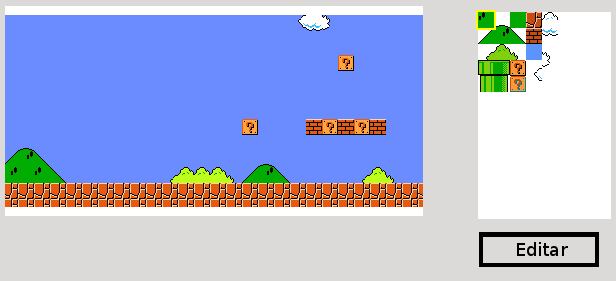
\includegraphics[width=\linewidth]{imgs/mockup.png}
\caption{Uma idéia da nossa interface} 
\end{figure}

Precisamos então decidir como faremos a interface. Como a parte do código da engine para o DS deverá ser feito em C++, pensamos que o ideal seria que o resto do projeto também fosse feito em C++, assim mantemos um certo padrão de linguagem. Com isso, buscamos as alternativas para a interface.

Como queremos que o projeto seja utilizável tanto em Windows, quanto em Linux, que será nossa principal plataforma de desenvolvimento, precisamos escolher uma biblioteca gráfica que suporte os dois sistemas operacionais e cujo custo de trocar de um pra outro seja muito baixo, ou seja, que não seja necessário reeescrever código para isso.

A solução que encontramos é utilizar a biblioteca Qt. A IDE para criação de interfaces, o QtCreator, deixa que as interfaces sejam criadas somente arrastando componentes e em seguida associando cliques a funções. E usando as funções do Qt para fazer as tarefas, o custo de troca entre Windows e Linux é basicamente zero. Falaremos mais sobre o porque da decisão da biblioteca no Anexo \ref{ferramentas-qt}.

Assim, fazemos a primeira janela do nosso programa, e o resultado é bem parecido com o que nós pensamos.

\begin{figure}[h!]
\centering
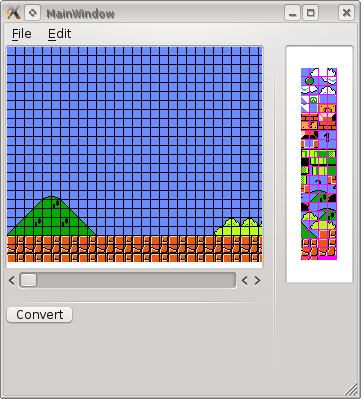
\includegraphics{imgs/mainwindow_1.png}
\caption{A nossa primeira interface} 
\end{figure}

Com a nossa interface definida, agora temos que nos preocupar em carregar o arquivo. Vamos considerar primeiro o problema de ler um arquivo já pronto e conversão desse arquivo para um formato do tipo ``mapa de tiles'', onde nós identificamos os tiles, e iremos compor o \textit{background} a partir desses tiles. Fazemos isso com o código \ref{list:tilesv1}.

Vamos entender o que fazemos nesse código. A leitura da imagem fica por conta do Qt. Preenchemos o fundo do grid que vai conter nosso \textit{background} com preto, em seguida, iteramos por toda a imagem, dividindo-a em quadrados de 8x8, ou seja, nossos tiles. Em cada um desses quadrados, identificamos se esse tile já foi incluído no nosso vetor de tiles. Se já, pegamos o índice desse vetor caso contrário, incluímos no vetor de tiles. Depois dizemos que nessa posição do \textit{background} está o tile com esse índice. 

Inicialmente, não deixamos que o usuário amplie o mapa, ou seja, a imagem que ele carregar inicialmente tem que ser composta por tiles e já do tamanho final do mapa. Nossa intenção para depois, no entanto, é que o usuário possa criar um mapa vazio e carregar somente o conjunto de tiles. Do contrário, nosso software se resumiria a ter a mesma função da ferramenta já existente, a PAGfx, somente com uma interface mais rebuscada.

Como já comentamos, o hardware do DS suporta que pedaços de mapa sejam espelhados, tanto na vertical quanto na horizontal. No nosso código, não tratamos nenhum desses casos. Esse problema será visto mais adiante. No momento estamos mais preocupados em ter algo que permita que exportemos os \textit{backgrounds} para que possamos começar a trabalhar na engine.

Agora que já lemos o \textit{background}, temos que implementar as seguintes funções: seleção de tiles, usar o tile selecionado para pintar no mapa e exportar o mapa para o formato do DS. Como já exibimos na pequena janela o tile, basta que associemos os eventos de clique à janela, para que possamos implementar a funcionalidade de seleção de tiles.

Nós em primeiro lugar fizemos um código bem rudimentar, que simplesmente achava a posição do tile a partir da posição que o usuário havia clicado, e desenhava um quadrado ao redor dessa posição. No entanto, ele desenhava múltiplos quadrados, no caso do usuário sair clicando, e não funcionava no caso em que o usuário clicava duas vezes no mesmo quadrado.

Mexemos no código até que o usuário pudesse selecionar um tile com um clique, e desfazer a seleção clicando novamente. E também passamos a guardar a informação sobre o índice do tile selecionado. Afinal, isso seria necessário para quando quiséssemos pintar usando o tile selecionado. Uma funcionalidade interessante seria selecionar grupos de tiles, mas nós decidimos não a implementar num primeiro momento.

Com isso, implementar o uso do tile para pintar no mapa era o próximo passo lógico. Tratamos disso fazendo a janela um pouco mais complexa, adicionamos um botão ``pintar'' e quando este botão está selecionado, o \textit{sprite} selecionado é usado para pintar na janela principal. Agora, já pensando em como faremos para exportar o mapa, precisamos tomar algumas medidas e refatorar algumas partes do código. Em primeiro lugar, como vimos anteriormente, vamos precisar de três partes: uma paleta de cores, os \textit{sprites} presentes, e um mapa desses \textit{sprites}. No momento nosso código não guarda nenhuma dessas informações. Então o que vamos refatorar é o código de leitura da imagem inicial.

Precisamos fazer com que ao ler a imagem, e processar os \textit{sprites}, sejam guardadas as cores que formos encontrando. Guardamos então essas cores num vetor, para que depois, quando formos processar a saída, possamos fazer os \textit{sprites} se relacionarem com essas cores. Os \textit{sprites} já estão guardados eles mesmos num vetor e o basta então que o fundo também seja armazenado numa matriz, relacionando-se com os \textit{sprites}.

Ao menos a princípio, escolhemos, como é comum em aplicações gráficas, o magenta para ser o transparente, ou seja, a primeira cor da paleta. Do mesmo modo, enquanto processamos as cores, já faremos a passagem para A1R5G5B5, que tem somente 5 bits de cor, ao contrário dos 8 que temos. Guardaremos então os 5 bits mais significativos. Veja a figura \ref{img:comparacao} para ter uma idéia da diferença que tirar os três bits menos significativos faz.

Ou seja, o procedimento passa a ser:

\lstinputlisting[caption=Pseudo-código de carregamento de arquivo,label=list:ploadfile]{codigos/pseudocodigo.c}

Com isso, chegamos basicamente onde queríamos chegar. Podemos agora usar o nosso programa para fazer o \textit{background} para ser testado no DS. Porém, falta ainda dar a saída para o formato da PALib. Mas agora isso é só uma questão de dar a saída do jeito certo, já que estamos com todos os dados preparados.

Fazemos isso com o seguinte código:

\lstinputlisting[caption=Pseudo-código de escrita de arquivo,label=list:pwritefile]
{codigos/pseudoescritacodigo.c}

Assim, agora podemos usar qualquer programa de edição de imagem para fazer os tiles, e em seguida, podemos usá-los para construir algum tipo de \textit{background} para a nossa engine. O DS suporta até cinco \textit{backgrounds} simultâneos, para que eles façam parallax ou simplesmente para dar ilusão de profundidade. Ainda não implementamos essa funcionalidade no nosso software, mas podemos circular essa limitação simplesmente editando os cinco \textit{backgrounds} em momentos diferentes.

\section{Engine: Movimento e colisões}

Agora, já tendo os meios para fazer o plano de fundo, é hora de voltar para a engine, começar a pensar no movimento básico do personagem principal, e nas colisões dele (e de outros personagens, como inimigos) com o ambiente. Nesse ponto, estamos observando as idéias mostradas em \cite[N Tutorial A]{NCollisionA} e \\\cite[N Tutorial B]{NCollisionB}.

Assim, a nossa idéia para a colisão foi de implementarmos, no mapa de tiles, quais tiles são sólidos e quais não são. Do mesmo modo, podemos fazer tiles que só são sólidos a partir de determinadas direções. Assim, podemos implementar plataformas onde o personagem consegue subir, mas uma vez em cima, não cai. Ao mesmo tempo, escolhemos como padrão para o personagem uma caixa envolvente em formato de pílula, assim como é feito pela Unity 3D.\footnotemark

Desse modo, nossa primeira preocupação é fazer a colisão entre o personagem e o mundo. Tentaremos fazer as rotinas o mais genéricas possíveis, para que possam ser aproveitadas para todos os nossos objetos dinâmicos. (Personagens, itens que andam e inimigos.)

\footnote{http://unity3d.com/ - Engine para jogos em 3D.}

\chapter{Ferramentas utilizadas}

Foi feita uma análise de algumas ferramentas que são muito usadas
por atacantes (hackers) para a confecção de ataques. Estas ferramentas
são muito úteis em vários aspectos, tais como: (1) o levantamento
de informações sobre o alvo, (2) que tipo de serviços estão disponíveis
no alvo, (3) quais as possíveis vulnerabilidades do alvo, entre outras
informações. As ferramentas analisadas foram o \emph{nmap}~,
o \emph{nessus}~, o \emph{saint}~, além
de alguns comandos de sistemas operacionais (UNIX-Like e Windows-Like)
usados para rede, tais como o \emph{ping, nslookup e whois}. 
\end{document}
